\documentclass[a4paper,12pt]{article}
\usepackage[
top=2.5cm,
bottom=2.5cm,
left=2cm,
right=2cm,
]{geometry}

\usepackage{enumitem}
\usepackage{amsmath,amssymb,latexsym}
\usepackage{pifont}

% Automata
\usepackage{tikz}
\usetikzlibrary{ arrows, automata, bbox, positioning}
\tikzset{
->, % makes the edges directed
>=stealth', % makes the arrow heads bold
node distance=3cm, % specifies the minimum distance between two nodes. Change if necessary.
every state/.style={thick}, % sets the properties for each ’state’ node
initial text=Start, % sets the text that appears on the start arrow
}

% No indentation
\setlength\parindent{0pt}

% Shorthand
\newcommand{\s}[1]{s_{#1}}
\newcommand{\caps}[1]{S_{#1}}
\newcommand{\ntxt}[1]{\footnotesize{#1}}

\begin{document}
\section{NFA to DFA}
In the following table, initial state is labeled with \(\rightarrow\) and final states are labeled with \(*\).
% The height of each row is set to 1.2 relative to its default height.
\renewcommand{\arraystretch}{1.2}
\begin{table}[h]
\centering
\begin{tabular}[tb]{r||l|l}
   state & 0 & 1 \\
  \hline
  \(\varnothing\) & \(\varnothing\) & \(\varnothing\) \\

  \(\rightarrow \{\s{0}\}\) & \(\varnothing\) & \(\{\s{1}\}\)\\

  \(\{\s{1}\}\) & \(\{\s{1}, \s{3}\}\) & \(\{\s{2}, \s{4}\}\) \\

  \(*\{\s{2}\}\) & \(\{\s{2}, \s{4}\}\) & \(\{\s{2}\}\) \\

  \(\{\s{3}\}\) & \(\{\s{4}\}\) & \(\{\s{0}, \s{3}\}\) \\

  \(\{\s{4}\}\) & \(\varnothing\) & \(\varnothing\) \\

  \(\{\s{1}, \s{3}\}\) & \(\{\s{1}, \s{3}, \s{4}\}\) & \(\{\s{0}, \s{2}, \s{3}, \s{4}\}\) \\

  \(*\{\s{2}, \s{4}\}\) & \(\{\s{2}, \s{4}\}\) & \(\{\s{2}\}\) \\

  \(\{\s{0}, \s{3}\}\) & \(\{\s{4}\}\) & \(\{\s{0}, \s{1}, \s{3}\}\) \\

  \(\{\s{1}, \s{3}, \s{4}\}\) & \(\{\s{1}, \s{3}, \s{4}\}\) & \(\{\s{0}, \s{2}, \s{3}, \s{4}\}\) \\

  \(*\{\s{0}, \s{2}, \s{3}, \s{4}\}\) & \(\{\s{2}, \s{4}\}\) & \(\{\s{0}, \s{1}, \s{2}, \s{3}\}\) \\

  \(\{\s{0}, \s{1}, \s{3}\}\) & \(\{\s{1}, \s{3}, \s{4}\}\) & \(\{\s{0}, \s{1}, \s{2}, \s{3}, \s{4}\}\) \\

  \(*\{\s{0}, \s{1}, \s{2}, \s{3}\}\) & \(\{\s{1}, \s{2}, \s{3}, \s{4}\}\) & \(\{\s{0}, \s{1}, \s{2}, \s{3}, \s{4}\}\) \\

  \(*\{\s{0}, \s{1}, \s{2}, \s{3}, \s{4}\}\) & \(\{\s{1}, \s{2}, \s{3}, \s{4}\}\) & \(\{\s{0}, \s{1}, \s{2}, \s{3}, \s{4}\}\) \\

  \(*\{\s{1}, \s{2}, \s{3}, \s{4}\}\) & \(\{\s{1}, \s{2}, \s{3}, \s{4}\}\) & \(\{\s{0}, \s{2}, \s{3}, \s{4}\}\) \\
\end{tabular}
\caption{The subset construction}
\end{table}

\section{DFA minimisation}
\renewcommand{\labelitemii}{\ding{226}}
\begin{enumerate}
% initial split
\item initial split: \(\{\s{1},\s{5}\}\), \(\{\s{0}, \s{2}, \s{3}, \s{4}\}\)
  \begin{itemize}
    \item check \(\{\s{1},\s{5}\}\)
      \begin{itemize}
      \item \(\s{1} \overset{0}{\rightarrow} \s{2}\), second group
      \item \(\s{5} \overset{0}{\rightarrow} \s{0}\), second group
      \item \(\s{1} \overset{1}{\rightarrow} \s{1}\), first group
      \item \(\s{5} \overset{1}{\rightarrow} \s{1}\), first group
      \item[] no split
    \end{itemize}

    \item check \(\{\s{0}, \s{2}, \s{3}, \s{4}\}\)
      \begin{itemize}
      \item \(\s{0} \overset{0}{\rightarrow} \s{1}\), first group
      \item \(\s{2} \overset{0}{\rightarrow} \s{5}\), first group
      \item \(\s{3}/\s{4} \overset{0}{\rightarrow} \s{4}\), second group
      \item \(\s{3} \overset{1}{\rightarrow} \s{3}\), second group
      \item \(\s{4} \overset{1}{\rightarrow} \s{0}\), first group
      \item[] split out \(\s{3}\) and \(\s{4}\)
    \end{itemize}
\end{itemize}

% 2nd split
\item next split: \(\{\s{1},\s{5}\}\), \(\{\s{0}, \s{2}\}\), \(\{\s{3}\}\), \(\{\s{4}\}\)
  \begin{itemize}
  \item check \(\{\s{1},\s{5}\}\)
    \begin{itemize}
      \item \(\s{1} \overset{0}{\rightarrow} \s{2}\), second group
      \item \(\s{5} \overset{0}{\rightarrow} \s{0}\), second group
      \item \(\s{1}/\s{5} \overset{1}{\rightarrow} \s{1}\), first group
      \item [] no split
    \end{itemize}
  \item check \(\{\s{0}, \s{2}\}\)
    \begin{itemize}
      \item \(\s{0} \overset{0}{\rightarrow} \s{1}\), first group
      \item \(\s{2} \overset{0}{\rightarrow} \s{5}\), first group
      \item \(\s{0}/\s{2} \overset{1}{\rightarrow} \s{3}\), third group
      \item[] no split
    \end{itemize}
  \item no need to check \(\{\s{3}\}\) or \(\{\s{4}\}\) alone
  \end{itemize}
\item Merge \(\s{1}\) and \(\s{5}\)
\item Merge \(\s{0}\) and \(\s{2}\)
\item Finally got \(\s{0}, \s{1}, \s{3}, \s{4}\)
\end{enumerate}

\section{\(\epsilon\)-NFA to NFA}
\subsection{\(\epsilon\)-closure}
\textbf{Solution.}
% step 1 find eclose of all states
\begin{itemize}
\item ECLOSE\((\s{0})\) = \(\{\s{0}, \s{1}, \s{4}, \s{2}\}\)
\item ECLOSE\((\s{1})\) = \(\{\s{1}, \s{4}, \s{2}, \s{0}\}\)
\item ECLOSE\((\s{2})\) = \(\{\s{2}\}\)
\item ECLOSE\((\s{3})\) = \(\{\s{3}\}\)
\item ECLOSE\((\s{4})\) = \(\{\s{4}, \s{2}, \s{0}, \s{1}\}\)
\end{itemize}
\subsection{Final NFA diagram}
\textbf{Solution.}\\
See diagram \ref{fig:nfa} on the next page.
% step 3 NFA
\clearpage
\begin{figure}[t]
  \centering
  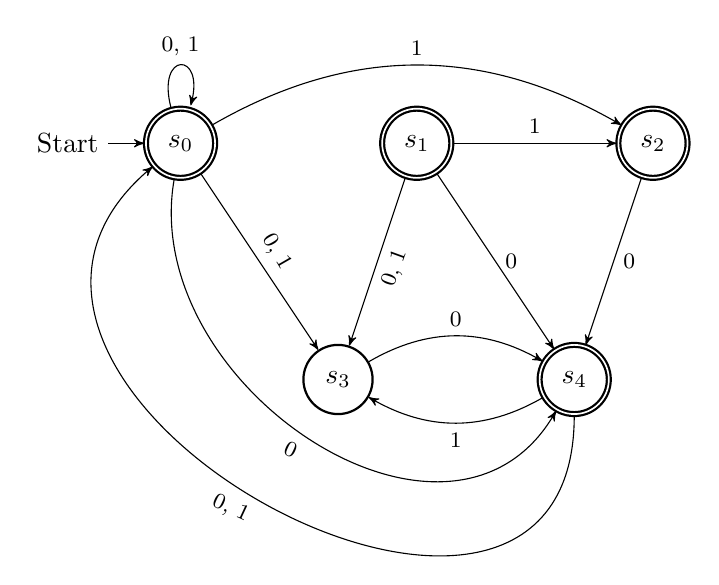
\begin{tikzpicture}[bezier bounding box]% reduce vertical spacing after tikzpicture
  \node[state, initial, accepting] (s0) {\(\s{0}\)};
  \node[state, accepting, right of=s0] (s1) {\(\s{1}\)};
  \node[state, accepting, right of=s1] (s2) {\(\s{2}\)};
  \node[state, right of=s0, xshift=-1cm, yshift=-3cm] (s3) {\(\s{3}\)};
  \node[state, accepting, right of=s3] (s4) {\(\s{4}\)};

  \draw (s0) edge[loop above] node{\ntxt{0, 1}} (s0)
             edge[bend left, above] node{\ntxt{1}} (s2)
             edge[above] node[rotate=-60]{\ntxt{0, 1}} (s3)
             edge[out=-100, in=-120, looseness=1.2] node[below left, rotate=-25]{\ntxt{0}} (s4)
        (s1) edge[above] node{\ntxt{1}} (s2)
             edge[below, right=0.3] node{\ntxt{0}} (s4)
             edge[below, right=0.3] node[below, rotate=70]{\ntxt{0, 1}} (s3)
        (s2) edge[below, right=0.3] node{\ntxt{0}} (s4)
        (s3) edge[bend left, above] node{\ntxt{0}} (s4)
        (s4) edge[bend left] node[below]{\ntxt{1}} (s3)
             edge[out=-90, in=-140, looseness=1.8] node[below left, rotate=-25]{\ntxt{0, 1}} (s0);
  \end{tikzpicture}
  \caption{NFA without \(\epsilon\)}
  \label{fig:nfa}
\end{figure}

\section{C++ streams}
\section{Deterministic Context Free Languages}
\end{document}
